\documentclass[a4paper, 12pt]{article}
\usepackage[top=2cm, bottom=2cm, left=2.5cm, right=2.5cm]{geometry}
\usepackage[utf8]{inputenc}
\usepackage[brazilian]{babel}
\usepackage{indentfirst}
\usepackage{graphicx}
\usepackage{wrapfig}
\usepackage[pdftex]{hyperref}
\graphicspath{ {imagens/} }
\usepackage{amsmath}

\begin{document}
%
\begin{titlepage} %iniciando a "capa"
	\begin{center} %centralizar o texto abaixo
		{\large Unicamp}\\[0.4cm] %0,2cm é a distância entre o texto dessa linha e o texto da próxima
		{\large Marco Lucio Bittencourt - Turma B}\\
		{\large Heitor Nigro Lopes - PED}\\[3.2cm]
		{\bf \huge Dinâmica Trabalho 2}\\[0.2cm] 
		{\bf \large Matrizes de Rotação e Range Kutta}\\[4.9cm]
		% o comando \bf deixa o texto entre chaves em negrito. O comando \huge deixa o texto enorme
	\end{center} %término do comando centralizar
	{\large Erik Yuji Goto}\\ % o comando \large deixa o texto grande
	RA: 234009\\[10cm]
	\begin{center}
	
		{\large Campinas}\\[0.2cm]
		{\large 2021}
	\end{center}
\end{titlepage} %término da "capa"


\tableofcontents
\newpage

\section{Observação}
	Não está englobado o material da P1
	\newpage
\section{Fasores}
	\begin{itemize}
		\item Resistor:\begin{equation}
			\underline{V_R} = R\underline{I_R}
		\end{equation}
		\item Indutor:\begin{equation}
			\underline{V_L} = j\omega L\underline{I_L}
		\end{equation}
		\item Capacitor:\begin{equation}
			\underline{V_C} = \frac{1}{j\omega C} \underline{I_C}
		\end{equation}
	\end{itemize}
	
\section{Impedância e Admitância}
	Define-se a impedância(Z) como a relação da tensão fasorial pela corrente fasorial:
	\begin{equation}
		Z = \frac{V_m}{I_m} \angle (\theta - \phi) = R + jX
	\end{equation}
	R é a componente resistivam e X é a componente reativa.\\
	A a admitância Y é o inverso da impedância.
	
	\begin{figure}[h]
		\centering
		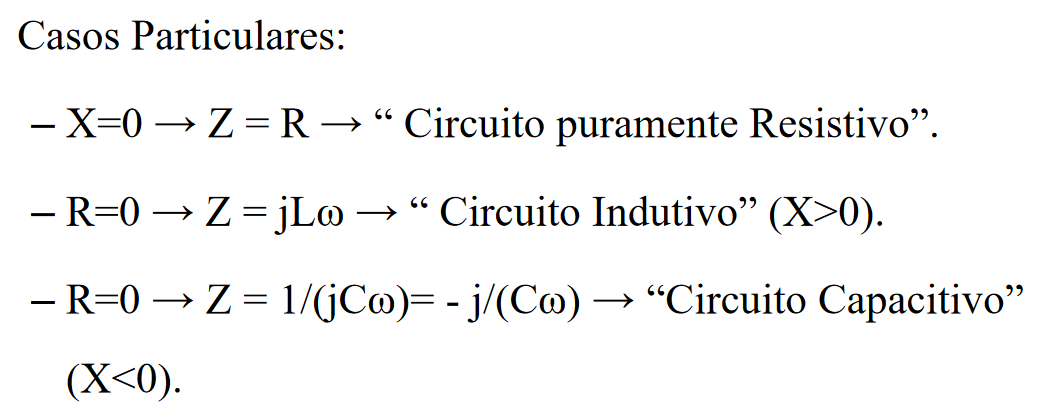
\includegraphics[scale=0.3]{a.png}
		\caption{Casos Particulares}
	\end{figure}
	
	\subsection{Associação de Impedâncias}
		\subsubsection{Série}
		\begin{equation}
			Z_{eq} = Z_1 + Z_2 + ... + Z_k 
		\end{equation}
		\subsubsection{Paralelo}
		\begin{equation}
			\frac{1}{Z_{eq}} = \frac{1}{Z_1} + \frac{1}{Z_2} + ... + \frac{1}{Z_k}
		\end{equation}
	
\section{Potência em excitações senoidais}
	\subsection{Potência Média}
		\begin{equation}
			\bar{p} = \frac{V_mI_m}{2} cos\theta
		\end{equation}
	
	\subsection{Valores Eficazes}
		O valor eficaz de uma corrente(tensão) periódica é equivalente a uma corrente(tensão) contínua que entrega a mesma potência média para um resistor:
		\begin{equation}
			I_{ef} = \frac{I_m}{\sqrt{2}}
		\end{equation}
		\begin{equation}
			V_{ef} = \frac{V_m}{\sqrt{2}}
		\end{equation}
		Portanto, a potência média fica:
		\begin{equation}
			\bar{p} = I_{ef} V_{ef} cos \theta
		\end{equation}
		Onde o produto $I_{ef}*V_{ef}$ é definido como a potência aparente.
		
	\subsection{Fator de Potência}
		O fator de potência ($f_p$) é definido como a relação entre a
potência média e a potência aparente:
		\begin{equation}
			f_p = cos\theta
		\end{equation}

		\begin{itemize}
			\item Carga RC - fator de potência adiantado;
			\item Carga RL - fator de potência atrasado;
		\end{itemize}
		Na prática é comum acrescentar um elemento puramente reativo (resistência nula) em paralelo com a impedância original, de modo a alterar o fator de potência ao nível desejado.

	\subsubsection{Correção do fator de Potência}
		Seja um sistema elétrico representado por uma impedância $Z= R + j X$. Suponha que em paralelo a esta
impedância é acrescentado o elemento $Z1= jX1$. Então, podemos calcular o valor da impedância em paralelo:
		\begin{equation}
			X_1 = \frac{R^2 + X^2}{R.tg(cos^{-1} f_p) - X}
		\end{equation}
		
	\newpage
	\subsection{Potência Complexa}
		A potência complexa é definida por:
		\begin{equation}
			S = \underline{V}_{ef}\underline{I}_{ef}^* = P + jQ
		\end{equation}
		$\underline{I}_{ef}^*$ é o conjugado da corrente eficaz.\\
		P é a potência ativa e Q a potência reativa.
		\begin{figure}[h]
			\centering
			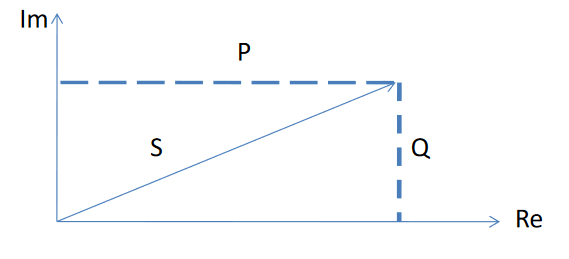
\includegraphics[scale=0.5]{a1.png}
			\caption{Potência Complexa}
		\end{figure}\\
		O módulo da potência complexa é dado por:
			\begin{equation}
				|S| = V_{ef}I_{ef}
			\end{equation}
		Que é igual à potência aparente. Então, a potência reativa Q é dada por:
			\begin{equation}
				Q = Im (S) = V_{ef}I_{ef}sin\theta
			\end{equation}
		Lembre que, a carga atendida é dada por:
			\begin{equation}
				Z = R + jX
			\end{equation}
	
	\subsection{Correção de $f_p$ em termos de potência}
		Uma potência complexa S é fornecido à carga Z. A potência fornecida pode ser decomposta em:
			\begin{equation}
				S = P + jQ
			\end{equation}
			Acrescenta-se uma carga de reatância pura Z1 em paralelo com Z. Com isso a potência complexa total fornecida ao circuito será:
			\begin{equation}
				S_T = P + j(Q + Q_1)
			\end{equation}

\section{Sistemas Trifásicos}
	Os sistemas trifásicos são constituídos de três sistemas monofásicos defasadas de 120. Usualmente as fases são nomeadas em a,b e c:
	\begin{figure}[h]
		\centering
		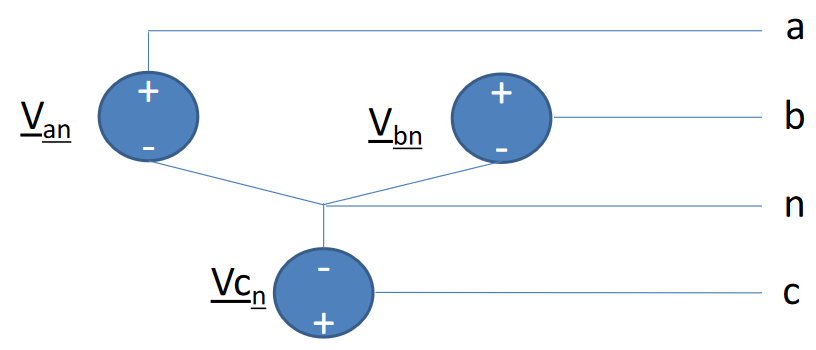
\includegraphics[scale=0.5]{a2.png}
		\caption{Sistema Trifásico}
	\end{figure}

	\begin{equation}
		v_a = V_p cos(\omega t) 
	\end{equation}
	\begin{equation}
		v_b = V_p cos(\omega t - 120)
	\end{equation}
	\begin{equation}
		v_c = V_p cos(\omega t + 120)
	\end{equation}

	\textbf{Tensão de Fase} é a tenão nos terminais das fontes trifásicas.
	\begin{equation}
		\underline{V_{an}} = V_p \angle 0
	\end{equation}
	\begin{equation}
		\underline{V_{bn}} = V_p \angle -120
	\end{equation}
	\begin{equation}
		\underline{V_{cn}} = V_p \angle 120
	\end{equation}

	\textbf{Tensão entre fases} é dado pela diferença de tensões de fase.
	\begin{equation}
		\underline{V_{ab}} = \sqrt{3}V_p \angle 30
	\end{equation}
	É importante destacar que no caso da tensão fasorial $\underline{V_{ab}}$ a
fase “a” é a referência. Com isso a fase do fasor da tensão entre as fases “a” e “b” é de 30º em relação à fase a.	
	
	De forma similar temos:
		\begin{equation}
			\underline{V_{bc}} = \sqrt{3}V_p \angle -90
		\end{equation}
		\begin{equation}
			\underline{V_{ca}} = \sqrt{3}V_p \angle 150
		\end{equation}

	\textbf{Convenção:}
	\begin{itemize}
		\item Os dados e variáveis relativos às conexões entre fontes e cargas são de linhas. Por exemplo, a corrente na conexão entre uma fonte e uma carga é dita corrente de linha;
		\item Os dados e variáveis relativos às fontes e cargas são de fase. Por exemplo, a tensão em uma carga é denominada tensão de fase.
	\end{itemize}

\newpage
\section{Conexão em Y-Y}
	\begin{figure}[h]
		\centering
		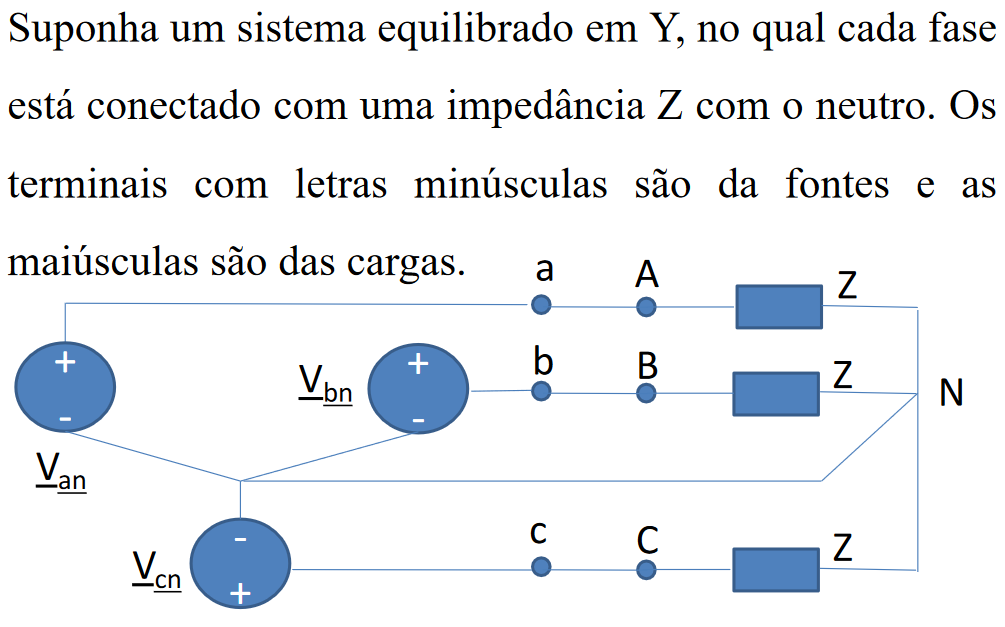
\includegraphics[scale=0.3]{a3.png}
		\caption{Conexão em Y-Y}
	\end{figure}
	Neste caso a impedância Z da fase A está conectada entre a saída da fonte a e o neutro. Então, a corrente sobre esta impedância é dada por:
	\begin{equation}
		\underline{I_{aA}} = \frac{\underline{V_{an}}}{Z} = I_{aA}\angle - \theta
	\end{equation}

	As correntes das outras cargas tem a mesma amplitude e com as fases defasadas de -120 e +120.
	\begin{equation}
		\underline{I_{bB}} = I_{aA} \angle (-120 - \theta)
	\end{equation}
	\begin{equation}
		\underline{I_{cC}} = I_{aA} \angle (120-\theta)
	\end{equation}

	Note que, numa conexão Y-Y equilibrada a quatro fios, a soma das três correntes de linha é nula. Portanto, a corrente pelo neutro é nula.\\
	
	A potência média entregur pela fase p é:
	\begin{equation}
		P_p = V_pI_p cos\theta
	\end{equation}
	Então a potência total entregue pelas 3 fases é:
	\begin{equation}
		P = 3P
	\end{equation}
	
\section{Conexão em Delta}
	\begin{figure}[h]
		\centering
		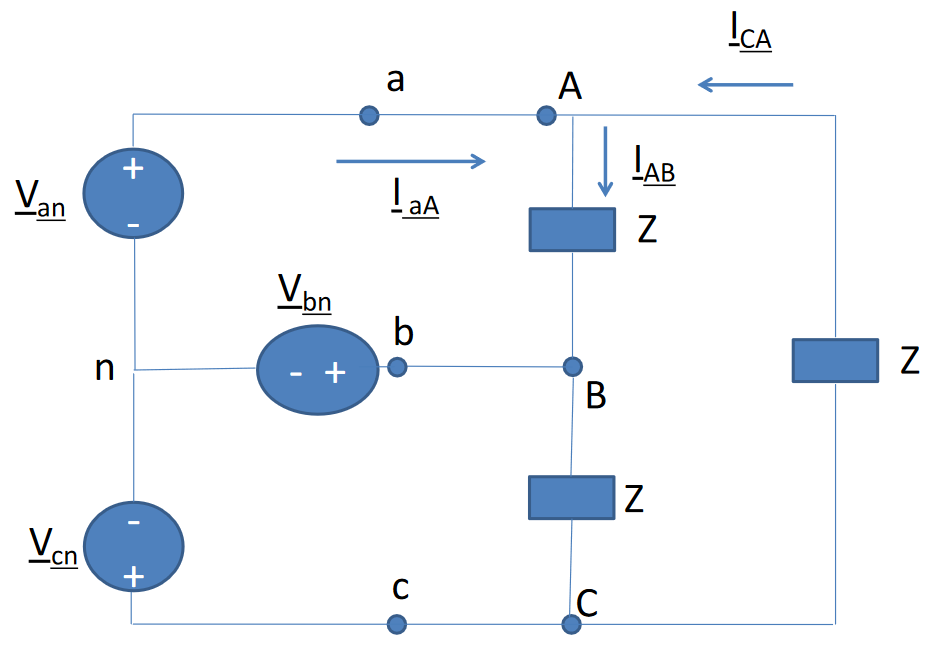
\includegraphics[scale=0.4]{a4.png}
		\caption{Conexão em Delta}
	\end{figure}
	\newpage
	Nesta configuração as impedâncias estão conectadas entre duas fases e não com o neutro.
	
	Já foi visto que as tensões entre fases são dadas por:
	\begin{equation}
		\underline{V_{AB}} = V_L \angle 30
	\end{equation}
	\begin{equation}
		\underline{V_{BC}} = V_L \angle -90
	\end{equation}
	\begin{equation}
		\underline{V_{CA}} = V_L \angle 150
	\end{equation}
	
	Onde,\\
	$V_L = \sqrt{3}V_p$\\
	
	As correntes de fase são dadas por:
	\begin{equation}
		\underline{I_{AB}} =  \frac{V_L \angle 30}{|Z| \angle \theta} = I_Z \angle(30 - \theta)
	\end{equation}
	\begin{equation}
		\underline{I_{BC}} =  \frac{V_L \angle -90}{|Z| \angle \theta} = I_Z \angle(-90 - \theta)
	\end{equation}
	\begin{equation}
		\underline{I_{CA}} =  \frac{V_L \angle 150}{|Z| \angle \theta} = I_Z \angle(150 - \theta)
	\end{equation}

	Por sua vez, a amplitude da corrente de linha é igual à corrente de fase multiplicada por $\sqrt{3}$. E a fase da corrente de linha é igual à fase da corrente na carga subtraída de 30º.
	\begin{equation}
		\underline{I_{aA}} = \sqrt{3}I_Z \angle -\theta
	\end{equation}
	\begin{equation}
		\underline{I_{bB}} = \sqrt{3}I_Z \angle (-120-\theta)
	\end{equation}
	\begin{equation}
		\underline{I_{cC}} = \sqrt{3}I_Z \angle (120-\theta)
	\end{equation}

\section{Transformação Y - $\Delta$}
	É possível transformar uma conexão de cargas equilibradas em Y em uma configuração equivalente em $\Delta$, ou vice-versa

	\subsection{Transformação de Y para $\Delta$}
		\begin{figure}[h]
			\centering
			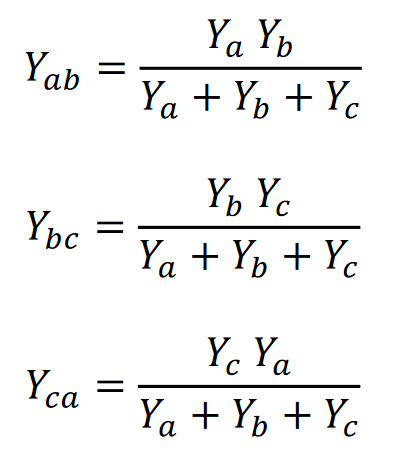
\includegraphics[scale=0.4]{a5.png}
			\caption{Transformação de Y para $\Delta$}
		\end{figure}
	\subsection{Transformação de $\Delta$ para Y}
		\begin{figure}[h]
			\centering
			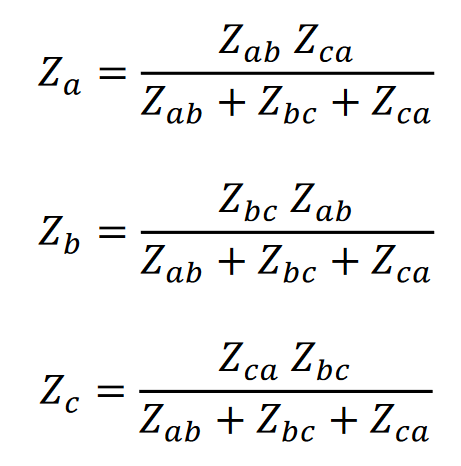
\includegraphics[scale=0.4]{a6.png}
			\caption{Transformação de $\Delta$ para Y}
		\end{figure}


\newpage
\section{Quadripolos}
	Um quadripolo é um circuito elétrico com dois pares de terminais, como ilustrado a seguir:
	\begin{figure}[h]
		\centering
		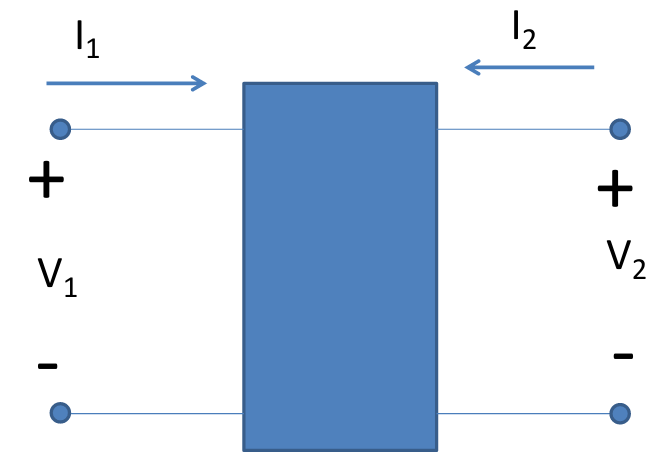
\includegraphics[scale=0.4]{a7.png}
		\caption{Convenção de um quadripolo}
		\label{quad}
	\end{figure}
	
	\subsection{Modelo de Impedâncias}
	Para este quadripolo adota-se o seguinte modelo:
	\begin{equation}
		V_1 = Z_{11}I_1 + Z_{12}I_2
		\label{quadmod1}
	\end{equation}
	\begin{equation}
		V_2 = Z_{21}I_1 + Z_{22}I_2
		\label{quadmod2}
	\end{equation}
	Os parâmetros podem ser obtidos por:
	\begin{equation}
		Z_{11} = \frac{V_1}{I_1} \textit{ (com $I_2$ = 0)}
	\end{equation}
	\begin{equation}
		Z_{21} = \frac{V_2}{I_1} \textit{ (com $I_2$ = 0)}
	\end{equation}
	\begin{equation}
		Z_{12} = \frac{V_1}{I_2} \textit{ (com $I_1$ = 0)}
	\end{equation}
	\begin{equation}
		Z_{22} = \frac{V_2}{I_2} \textit{ (com $I_1$ = 0)}
	\end{equation}

	$Z_{11}$ e $Z_{22}$ são as impedâncias vistas pela entrada e pela saída respectivamente.\\
	$Z_{12}$ e $Z_{21}$ são as impedâncias de transferências.
	
	\subsection{Modelo de Admitância}
	\begin{equation}
		I_1 = Y_{11}V_1 + Y_{12}V_2
	\end{equation}
	\begin{equation}
		I_2 = Y_{21}V_1 + Y_{22}V_2
	\end{equation}

	Calculo de parâmetros de curto circuito($V_1 = 0$ ou $V_2 = 0$):
	\begin{equation}
		Y_{11} = \frac{I_1}{V_1} \textit{ (com $V_2 = 0$)}
	\end{equation}
	\begin{equation}
		Y_{12} = \frac{I_1}{V_2} \textit{ (com $V_1 = 0$)}
	\end{equation}
	\begin{equation}
		Y_{21} = \frac{I_2}{V_1} \textit{ (com $V_2 = 0$)}
	\end{equation}
	\begin{equation}
		Y_{22} = \frac{I_2}{V_2} \textit{ (com $V_1 = 0$)}
	\end{equation}

	\subsection{Modelos com Parâmetros de Trnasmissão}
	Seja o modelo a seguir:
		\begin{equation}
			V_1 = AV_2 - BI_2
		\end{equation}
		\begin{equation}
			I_1 = CV_2 - DI_2
		\end{equation}
		Estes modelos são úteis em circuitos em cascata.

	\subsection{Cálculo de ganhos}
		Usando o modelo da figura \ref{quad} e equações \ref{quadmod1} e \ref{quadmod2}, define-se o ganho de tensão (GT) por $GT = \frac{V_2}{V_1}$, com $I_2 = 0$. Ou seja,\\
		\begin{equation}
			GT = \frac{V_2}{V_1} = \frac{Z_{21}}{Z_{11}}
		\end{equation}
		Define-se o ganho de corrente como $GC = \frac{I_2}{I_1}$, com $V_2 = 0$,
		\begin{equation}
			GC = \frac{Y_{21}}{Y_{11}}
		\end{equation}\\
		
		Cálculo de ganhos considerando\textit{ impedância interna }do gerador e carga:	
		\begin{figure}[h]
			\centering
			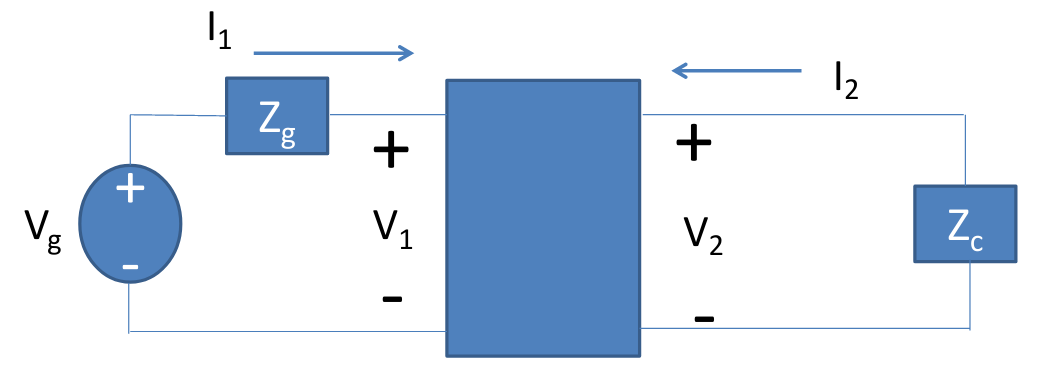
\includegraphics[scale=0.4]{a8.png}
			\caption{Quadripolo}
		\end{figure}	

		\begin{equation}
			\frac{V_2}{V_g} = \frac{Z_{21}Z_C}{(Z_{11} + Z_g)(Z_{22} + Z_c) - Z_{12}Z_{21}}
		\end{equation}
		\begin{equation}
			\frac{I_2}{I_1} = \frac{-Z_{21}}{Z_{22} + Z_c}
		\end{equation}

	\newpage
	\subsection{Circuitos Equivalente}
		Um quadripolo pode ser substituído por um circuito com fontes vinculadas:
		\begin{figure}[h]
			\centering
			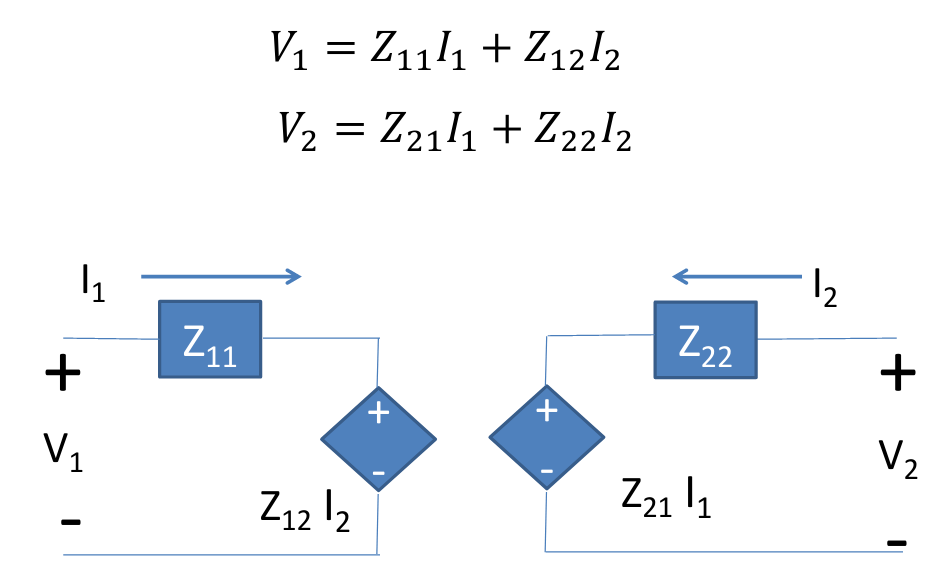
\includegraphics[scale=0.4]{a9.png}
			\caption{Quadripolo -> Fonte vinculada}
		\end{figure}
		
	\subsection{Associação em paralelo}
		\begin{figure}[h]
			\centering
			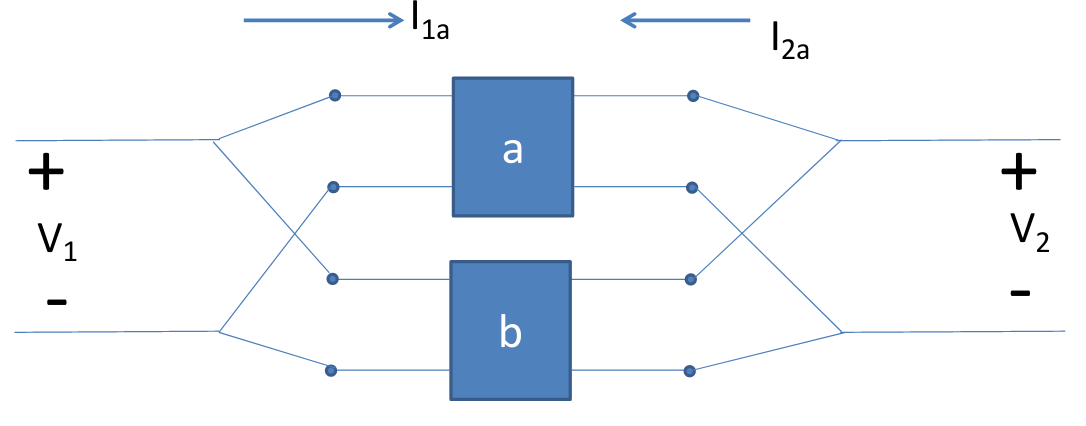
\includegraphics[scale=0.4]{a10.png}
			\caption{Associação em paralelo}
		\end{figure}
		\begin{equation}
			I_1 = (Y_{11a} + Y_{11b})V_1 + (Y_{12a} + Y_{12b})V_2
		\end{equation}
		\begin{equation}
			I_2 = (Y_{21a} + Y_{21b})V_1 + (Y_{22a} + Y_{22b})V_2
		\end{equation}
		
		Ou seja, nas associações em paralelo de quadripolos, no modelo com admitâncias, soma-se as admitâncias dos quadripolos da associação.
		
		\newpage
		\subsection{Associação em série}
		\begin{figure}[h]
			\centering
			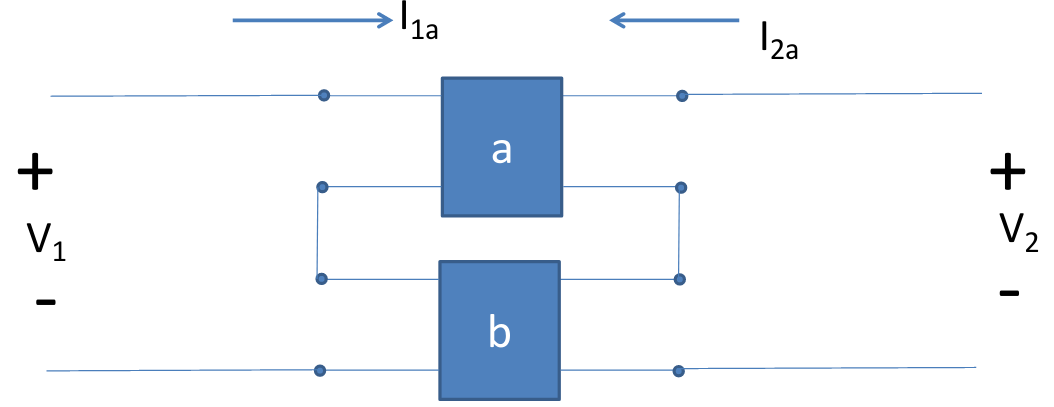
\includegraphics[scale=0.4]{a11.png}
			\caption{Associação em série}
		\end{figure}
		\begin{equation}
			V_1 = (Z_{11a} + Z_{11b})I_1 + (Z_{12a} + Z_{12b})I_2
		\end{equation}
		\begin{equation}
			V_2 = (Z_{21a} + Z_{21b})I_1 + (Z_{22a} + Z_{22b})I_2
		\end{equation}
		
		Ou seja, nas associações em série de quadripolos, no modelo com impedâncias, soma-se as impedâncias dos quadripolos da associação.

		\subsection{Associação em cascata}
		\begin{figure}[h]
			\centering
			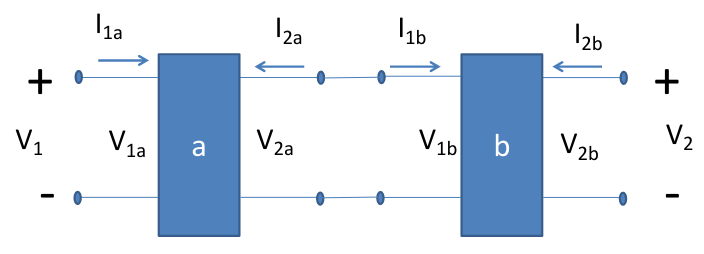
\includegraphics[scale=0.4]{a12.png}
			\caption{Associação em cascata}
		\end{figure}
		Seja o modelo de transmissão:
		\begin{equation}
			V_1 = AV_2 - BI_2
		\end{equation}
		\begin{equation}
			I_1 = CV_2 - DI_2
		\end{equation}
		Donde tem-se:
		\begin{equation}
			V_1 = (A_aA_b + B_aC_b)V_2 - (A_aB_b+B_aD_b)I_2
		\end{equation}
		\begin{equation}
			I_1 = (C_aA_b + D_aC_b)V_2 - (C_aB_b+D_aD_b)I_2
		\end{equation}
		Este modelo pode ser reescrito em termos de parâmetros
de transmissão equivalentes:
		\begin{equation}
			V_1 = A_{eq}V_2 - B_{eq}I_2
		\end{equation}
		\begin{equation}
			I_1 = C_{eq}V_2 - D_{eq}I_2
		\end{equation}

		Onde,
		\begin{equation}
			\begin{bmatrix}
				A_{eq} & B_{eq}\\
				C_{eq} & D_{eq}				
			\end{bmatrix} = \begin{bmatrix}
			A_a & B_a \\
			C_a & D_a
			\end{bmatrix}
			\begin{bmatrix}
			A_b & B_b\\
			C_b & D_b
			\end{bmatrix}
		\end{equation}

\section{Transformadores}
Os transformadores em circuitos elétricos são importantes pois possibilitam a transmissão em alta tensão, viabilizando a transmissão a longa distância.\\

Um dos enrolamentos é conectado a uma \textit{fonte}; este enrolamento é denominado o \textbf{primário} do transformador. O outro terminal é dito o \textbf{secundário}, ao qual usualmente se conecta a \textit{carga}.
	\subsection{Primário e secundário em carga}
		Quando tanto o primário como o secundário estão com correntes não nulas, então o fluxo magnético total em cada um dos enrolamentos é composto do fluxo gerado no próprio enrolamento e do fluxo mútuo recebido do outro enrolamento. E temos as seguintes equações:
		\begin{equation}
			v_1 = L_1\frac{d_1}{dt} + M\frac{di_2}{dt}
		\end{equation}
		\begin{equation}
			v_2 = M\frac{d_1}{dt} + L_2\frac{di_2}{dt}
		\end{equation}
		
		\subsection{Convenção do ponto}
		\begin{quote}
			Uma corrente i que entra num terminal com ponto (sem ponto) em um enrolamento induz uma tensão $M\frac{di}{dt}$ com polaridade positiva no terminal com ponto (sem ponto)
do outro enrolamento.
		\end{quote}
		
		\subsection{Impedância Refletida}
		Seja o seguinte circuito
		\begin{figure}[h]
			\centering
			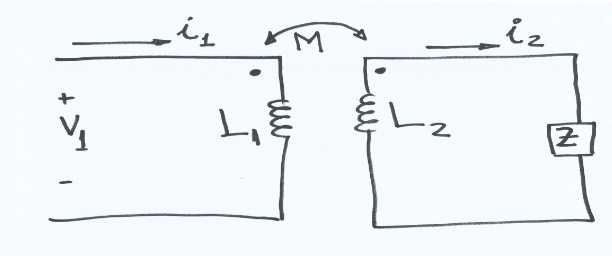
\includegraphics[scale=0.4]{a13.png}
			\caption{Impedância Refletida}
		\end{figure}\\
		O modelo do circuito é:
		\begin{equation}
			\underline{V_1} = j\omega L_1 \underline{I_1} - j\omega M \underline{I_2}
		\end{equation}
		\begin{equation}
			0 = -j\omega M \underline{I_1} + (Z + j \omega L_2)\underline{I_2}
		\end{equation}\\
		Donde tem-se que:
		\begin{equation}
			\underline{V_1} = (j\omega L_1 + \frac{\omega^2 M^2}{Z + j\omega L_2})\underline{I_1}
		\end{equation}
		Assim, a impedância vista pelos terminais do primário, a impedância equivalente, será:
		\begin{equation}
			\underline{Z_e} = j\omega L_1 + \frac{\omega^2 M^2}{Z + j\omega L_2}
			\label{eq}
		\end{equation}
		O primeiro termo é a impedância própria e o segundo termo é a impedância do acoplamento, também conhecido como impedância refletida. Ela representa a carga adicional para o primário devido ao acoplamento eletromagnético e à carga Z do secundário.
		
	\subsection{Circuitos Equivalentes}
		\subsubsection{Circuito 1}
			Como a impedância equivalente (\ref{eq}) leva em conta o acoplamento eletromagnético e a carga no secundário, então o circuito com o transformador e carga pode ser representado de forma equivalente pelo circuito mostrado na figura a seguir:
			\begin{figure}[h]
				\centering
				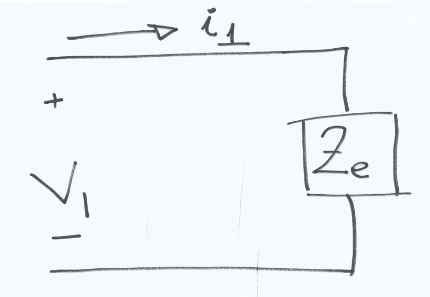
\includegraphics[scale=0.4]{a14.png}
				\caption{Circuito 1}
			\end{figure}\\
		\subsubsection{Circuito 2}
			Sejam as equações a seguir:
			\begin{equation}
				v_1 = L_1 \frac{i_1}{dt} + m \frac{di_2}{dt}
			\end{equation}
			\begin{equation}
				v_2 = M \frac{i_1}{dt} + L_2 \frac{di_2}{dt}
			\end{equation}
			\begin{figure}[h]
				\centering
				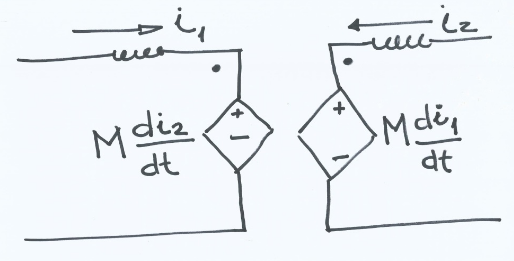
\includegraphics[scale=0.4]{a15.png}
				\caption{Circuito 2}
			\end{figure}\\
		\subsubsection{Circuito 3}
			\begin{equation}
				v_1 = (L_1 - M)\frac{di_1}{dt} + M (\frac{di_1}{dt} + \frac{di_2}{dt})
			\end{equation}
			\begin{equation}
				v_2 = M(\frac{di_1}{dt} + \frac{di_2}{dt}) + (L_2 - M) \frac{di_2}{dt}
			\end{equation}\\
			\newpage
			\begin{figure}[h]
				\centering
				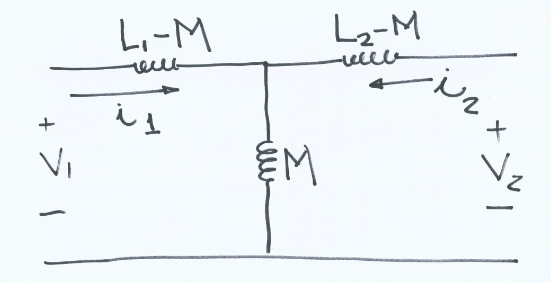
\includegraphics[scale=0.4]{a16.png}
				\caption{Circuito 3}
			\end{figure}
			
	\subsection{Armazenamento de Energia em Transformadores}
		Sejam duas bobinas acopladas conforme a figura a seguir.
		\begin{figure}[h]
			\centering
			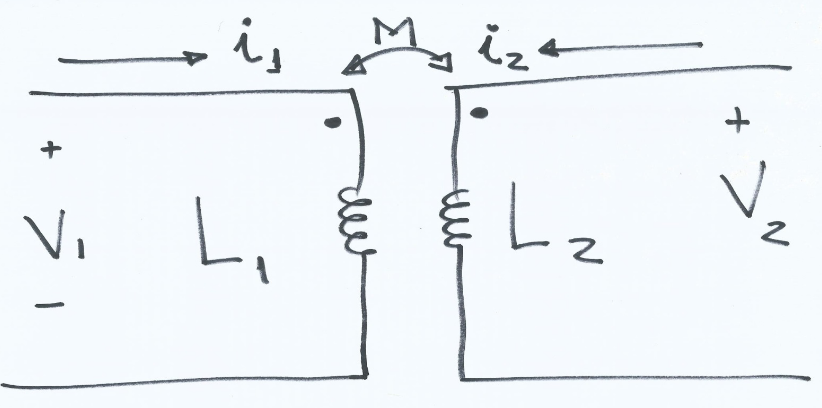
\includegraphics[scale=0.4]{a17.png}
			\caption{Bobinas Acopladas}
		\end{figure}
		A energia total fornecida pelos terminais é:
		\begin{equation}
			w = \frac{1}{2}L_1I_1^2 \pm MI_1I_2 + \frac{1}{2} L_2I_2^2
		\end{equation}
		O sinal de M depende da configuração de pontos.
		
	\subsection{Coeficiente de Acoplamento}
		Define-se o coeficiente de acoplamento por:
		\begin{equation}
			k = \frac{M}{\sqrt{L_1L_2}}
		\end{equation}
		Onde, \\
		$0 \leq k \leq 1$, quando k = 0 as bobinas não são acopladas, e k = 1 são totalmente acopladas.
		Se $k \leq 0.5$ é dito fracamente acolpada, e se $k > 0.5$ é fortemente acoplado. Portanto, os limites de acoplamento são:
		\begin{equation}
			0 \leq M \leq \sqrt{L_1L_2}
		\end{equation}

	\newpage1
	\subsection{Transformador Ideal}
		Um transformador ideal tem as seguintes características:
		\begin{enumerate}
			\item Sem perdas;
			\item Acoplamento unitário;
				\begin{equation}
					M = \sqrt{L_1L_2}
				\end{equation}
			\item Indutâncias próprias infinitas, mas sua relação é finita.
		\end{enumerate}
		Além disso, temos:
			
			\begin{equation}
				\frac{L_2}{L_1} = (\frac{n_2}{n_1})^2 = n^2
			\end{equation}
			\begin{equation}
				\frac{\underline{V_2}}{\underline{V_1}} = n
			\end{equation}
			\begin{equation}
				\frac{\underline{I_2}}{\underline{I_1}} = \frac{1}{n}
			\end{equation}
			\begin{figure}[h]
				\centering
				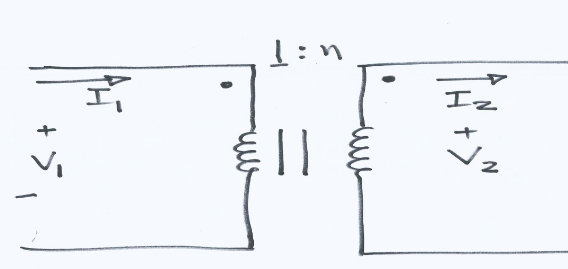
\includegraphics[scale=0.4]{a18.png}
				\caption{Transformador Ideal}
			\end{figure}\\
Para esta configuração de pontos e de correntes as relações são para n positivo. Uma alteração nesta configuração torna as relações negativas (-n)
\newpage
\section{Banco de Transformadores}
	\subsection{Conexão Y-Y}
		\begin{figure}[h]
			\centering
			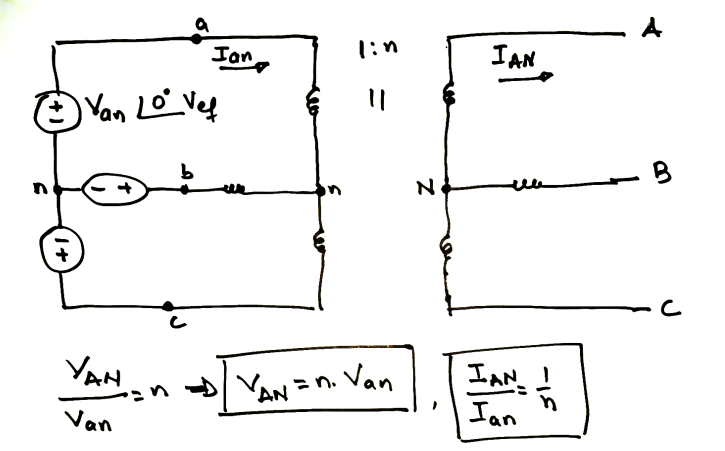
\includegraphics[scale=0.6]{a19.png}
			\caption{Y-Y}
		\end{figure}

	\subsection{Conexão Y-Delta}
		\begin{figure}[h]
			\centering
			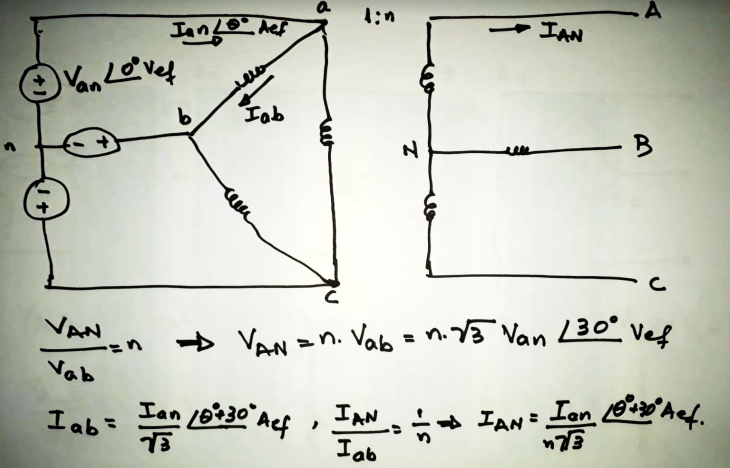
\includegraphics[scale=0.6]{a20.png}
			\caption{Y-Delta}
		\end{figure}



\end{document}
